\documentclass[a4paper]{article}

\usepackage[english]{babel}
\usepackage[utf8]{inputenc}
\usepackage{amsmath}
\usepackage{listings}
\usepackage{color}
\usepackage{hyperref}
\usepackage{float}
\usepackage{graphicx}
\graphicspath{{../pics/}}

\title{Machine Learning (course 1DT071)
Uppsala University – Spring 2015
Report for Assignment 3 by group 2}

\author{Ludvig Sundstr\"{o}m and John Shaw}
\date{\today}

\begin{document}

\maketitle

\section*{Task 1: Training on simple 3-dimensional data}

\subsection*{Question 1} 

\emph{Use } \texttt{plotsomehits} \emph{ to study the overlap between the winning nodes for the two clusters, as above. What amount of overlap do you see for each different data set?}

% \begin{figure}[H] %float here
	% 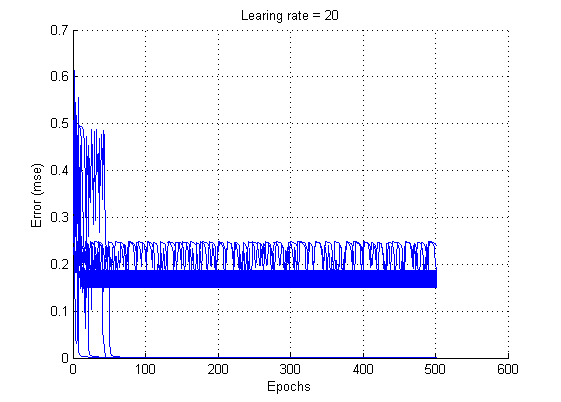
\includegraphics[]{plot2_LR20.png}
	% \caption{\label{fig:plot2_LR20}\textbf{Plot 1} from 10 Training sessions with a learning rate of 20.}
% \end{figure}

\textbf{Answer:} As the sparseness increases, the amount of overlap between the clusters increases as well.

%insert plot 1: plotsomehits figures for cluster F1 both with P10 som_P30 and P30 with som_P10

\subsection*{Question 2}
\emph{Explain why the two }\texttt{plotsomhits} \emph{ figures that you created for Plot 1 look the way they do.}

\textbf{Answer:} som\_10-P30 displays the winning nodes of the SOM trained on the most dense data applied on the most sparse data. Since the data is much more sparse than the distribution of nodes, the nodes on the edge of the map is most likely to win. som\_30-P190 displays the winning nodes of the SOM trained on the most sparse data applied on the most dense data. Here, a couple nodes inside the map close to the dense cluster are most likely to win. 

%insert plot 2: The smoothest RGB map we could produce

\section*{Task 2: Mapping of RGB color data}

\subsection*{Question 3}
\emph{What relation between the ordering phase and tuning phase seems to be best in order to get a smooth map? Why do you think that is?}

\textbf{Answer:} 
In this problem, the data lies in 3-dimensional space. How can we make the map cover the data in a good way? We can think of the 2-dimensional map as a paper arc which is formed  in some way to occupy as much space as possible in a 3D-cube. Even though we want to map a good variation of colors, it is more important to have smooth transitions between nodes in this problem. With this in mind, it would be good to form the map as a globe occupying as much as possible of the 3D-cube. In essence, this problem is to minimize the difference of the distances between the nodes. In order to do this, we found that we needed to train the network with no tuning phase at all. If we added a tuning phase where the nodes are moved individually, the distances start to differ and the shape of the map was distorted, resulting in a non-smooth color plot.

\subsection*{Question 4}
\emph{What training parameters did you use? How well does the trained
SOFM separate the classes in your opinion? Is some class easier to separate then the rest? If so, which one?}

\textbf{Answer:} We trained the map for 200 epochs in total with only one epoch in ordering phase. The first class was easier to separate from the others. The SOFM performed quite badly. 

\subsection*{Question 5}
\emph{What training parameters did you use? What  major differences
do you see in the results compared to the 5 by 5-node SOFM?}

\textbf{Answer:} This time we used a 10 times 10 network and the same parameters except that we changed the total number of epochs to 300. One major difference is that we get better precision in the classification since 25 nodes was not enough to cover the training data. With 100 nodes we get better coverage over the first cluster that is less dense than the other two classes. The other two classes are more dense and they are overlapping a bit. We got a better cover over the area with these two nodes as well and that helped to separate them as well.

\subsection*{Question 6}
\emph{How well do the SOFM separate the classes in the normalized
data?}

\textbf{Answer:} 
Pretty damn good.

\section*{Task 4: Analysis of flower data}

\subsection*{Question 7}
\emph{How well does the SOFM separate the classes, in your opinion?}

\textbf{Answer:} 

\subsection*{Question 8}
\emph{f you did not already know that the data came from three different species of Iris flowers, could you have found any evidence in the neighbor
distances plot to indicate that the data are not from a single species? What evidence would that be, and what does it imply about the distribution of the data?
Describe your reasoning.}

\textbf{Answer:} 

\subsection*{Question 9}
\emph{Do any of the attributes seem particularly correlated? Which
ones? Explain your reasoning.}

\textbf{Answer:} 

\subsection*{Question 10}
\emph{Which species has the smallest petals? Which species has the
largest petals? Explain your reasoning.}

\textbf{Answer:} 

\section*{Task 5: Analysis of unknown data}

\subsection*{Question 11}
\emph{How many well-separated clusters are there in the data set?
Explain how you found out your answer. Include figures if necessary.}

\textbf{Answer:} 

\subsection*{Question 12}
\emph{Which data points are from the same cluster? How did you
figure it out? Include figures if necessary.} 

\textbf{Answer:}

\section*{Task 6: Wrapping up}

\subsection*{Question 13}
\emph{Propose a real-world problem that you consider interesting and
that you believe can be solved using a SOFM. Explain in a few sentences how the
SOFM would be used, and what kind of data that it would be trained on.}

\textbf{Answer:} 

\end{document}
